\documentclass[a4paper,conference]{IEEEtran}
\usepackage{graphicx}
\usepackage{amsmath}
\usepackage{url}

\makeatletter
\newcommand{\authornewline}{
        \end{@IEEEauthorhalign}
        \hfill\mbox{}\par\mbox{}\hfill
        \begin{@IEEEauthorhalign}
}
\makeatother

\author{
    \IEEEauthorblockN{Hernán Alejandro Silva}
    \IEEEauthorblockA{
        Facultad Regional Avellaneda\\
        Universidad Tecnológica Nacional\\
        Buenos Aires, Argentina\\
        hernansilva2002@gmail.com
    }
    \and
    \IEEEauthorblockN{Elías Ramírez}
    \IEEEauthorblockA{
        Facultad Regional Avellaneda\\
        Universidad Tecnológica Nacional\\
        Buenos Aires, Argentina\\
        foo@gmail.com
    }
    \and
    \IEEEauthorblockN{Florencia Mincone}
    \IEEEauthorblockA{
        Facultad Regional Avellaneda\\
        Universidad Tecnológica Nacional\\
        Buenos Aires, Argentina\\
        foo@gmail.com
    }
    \authornewline
    \IEEEauthorblockN{Nicolás Lahorca}
    \IEEEauthorblockA{
        Facultad Regional Avellaneda\\
        Universidad Tecnológica Nacional\\
        Buenos Aires, Argentina\\
        foo@gmail.com
    }
    \and
    \IEEEauthorblockN{Luciano Justiniano}
    \IEEEauthorblockA{
        Facultad Regional Avellaneda\\
        Universidad Tecnológica Nacional\\
        Buenos Aires, Argentina\\
        foo@gmail.com
    }
}
\title{Detector de Partículas Beta}

\begin{document}
\maketitle
\begin{abstract}
    Constantemente los objetos que nos rodean emiten partículas que los sentidos
    humanos no son capaces de percibir. Estas partículas pueden ser
    perjudiciales para la salud y es necesario cuantificarlas y/o detectarlas
    para evitar o reducir la exposición a ellas. Para lograr ese objetivo, en
    este documento se presenta la realización de un dispositivo que cumpla la
    función de detectar un tipo de radiación, llamada radiación
    $\boldsymbol{\beta}$. En particular, se hará hincapié en la radiación por
    emisión de electrones, a este tipo de radiación se la conoce como radiación
    $\boldsymbol{\beta-}$. Además, se propone el análisis de su principio de
    funcionamiento, los materiales necesarios para su construcción y sus
    limitaciones.
\end{abstract}
\section{Introducción}
    El presente documento sirve como informe sobre el proyecto de fin de año de
    la asignatura Física Electrónica. Dicho proyecto se trata de un detector y
    contador de partículas beta, cubriendo de esta forma el tema de "Radiación"
    de la asignatura. Para más información sobre el proyecto, se recomienda
    visitar el repositorio del mismo que se encuentra en el siguiente enlace:
    (enlace al repo del proyecto).
\section{Principio de Funcionamiento}
    \subsection{¿Que son las radiaciones $\beta$?}
        Las radiaciones $\beta$ son un tipo de radiacion ionizante, la cúal se
        caracteriza por emitirse durante el proceso de desintegración o
        decaimento $\beta$. Dicho proceso puede producirse de dos diferentes
        formas.
        \begin{enumerate} 
            \item \textit{Emisión de electrones}: Un núcleo inestable de un
                átomo emite un electrón y un antineutrino, conviritiendo de esta
                manera un neutrón en un protón como \emph{Desintegración $\beta+$}.
            \item \textit{Emisión de positrones}: El núcleo inestable emite un
                positrón, es decir, un electrón cargado positivamente, junto con
                un neutrino. De esta forma se logra transformar un protón en un
                neutrón. Este proceso recibe el nombre de
                \emph{Desintegración $\beta+$}. 
        \end{enumerate}

        Generalmente, las fuentes más comunes de radiación de partículas $\beta$
        son piedras con pequeñas cantidades de uranio, y diferentes fuentes de
        potasio, como el cloruro de potasio (KCl), el cúal contiene baja
        cantidad del isótopo potasio 40 (K40), capáz de emitir partículas
        $\beta-$.

    \subsection{Formas de captar las partículas}
       El dispositivo electrónico más estudiado y utilizado para detectar la
       radiación de diferentes tipos de partículas es el diodo PIN o fotodiodo.
       Como muestra la figura \ref{fig:pin}, este es similar en cuanto a
       estructura a un diodo de juntura PN, la diferencia radica en que el PIN
       tiene una zona de material semiconductor intrínseco (zona I) entre la
       zona dopada positivamente (zona P) y la zona dopada negativamente (zona
       N).\par Al ser un material semiconductor, la zona I contiene átomos de
       silicio que, al momento de ser impactados por una partícula irradiada
       debido a una fuente radioactiva, genera la rotura de los enlaces
       covalentes del átomo, produciendo un \emph{par electrón-laguna}. La
       generación de este par tiene como consecuencia un pulso de corriente de
       decenas hasta cientos de microampere que atraviesan al diodo. Esta
       corriente puede ser medida. Cuando al diodo se lo polariza en
       forma inversa (cátodo con potencial más alto que el del ánodo),
       se generan dos regiones de vaciamiento: La primera se encuentra
       localizada entre la zona P y la zona I, y la otra entre dicha zona
       intrínseca y la zona N; en estas regiones, no se encuentran portadores
       libres, sino que exisen iones fijos cargados positiva y negativamente.
       Estos iones fijos son los responsables que en dichas regiones se encuentre
       un campo eléctrico, el cúal atrapa e impulsa a los portadores, aumentando
       la intensidad de corriente eléctrica a través del diodo.
       \newpage
       \begin{figure}[!t]
           \centering
           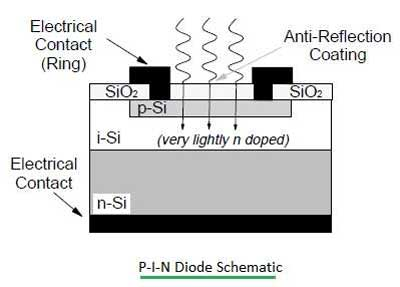
\includegraphics[width=2.5inch]{img/PIN_structure.jpg}
           \caption{Corte transversal de una estructura típica del diodo PIN}
           \label{fig:pin}
       \end{figure}
    \subsection{El fotodiodo como detector de partículas $\beta$}
        La zona intrínseca explicada anteriormente es conocida como \emph{zona
        sensible}, porque es donde las partículas irradiadas impactan. Como se
        menciona en \cite{mpdi}, las zonas sensibles de los fotodiodos son
        capaces de absorber algunos tipos de radiaciones ionizantes. La
        detección de las partículas que impactan está directamente relacionada
        con la profundidad de la zona sensible del diodo; esta zona (región de
        vaciamiento) aumenta de profundidad al elevar el voltaje de polarización
        inversa del dispositivo, dicha relación responde matemáticamente a

        \begin{equation}
            \label{d_x}
            d(V) = \frac{\epsilon_{r}\epsilon_{0}A}{C(V)}
        \end{equation}

        \hfill \\ donde:
        \begin{itemize}
            \item d(V) es la profunidad de la zona sensible.
            \item $\epsilon_{r}$ es la permitividad relativa del material, en este caso el Si
                (silicio).
            \item $\epsilon_{0}$ es la permitividad del vacío.
            \item A es el área física de la zona sensible del diodo.
            \item C(V) es la capacitancia del diodo a un determinado nivel de
                voltaje de polarización inversa.
        \end{itemize}

        Este valor de profundidad permite conocer la energía cinética máxima que
        se puede detectar de una partícula. Como se mencionó anteriormente, los
        valores de interés corresponden a partículas $\beta-$ (electrones). Para
        establecer el valor de energía mencionado, es necesario conocer la
        magnitud del rango \emph{CSDA (continuos slowing down approximation)}.
        El rango CSDA es una aproximación muy cercana del promedio de longitud
        de una trayectoria que recorre una partícula cargada a medida que se
        frena hasta alcanzar el reposo \cite{nist}. Para los electrones, los
        valores del CSDA están tabulados en \cite{nist}.\par
        Para obtener una medición fiable, es necesario que el rango CSDA sea
        menor que la profundidad de la zona sensible del diodo; esto es

        \begin{equation*}
            R_{p} < d(V)
        \end{equation*}

        \hfill \\ donde $R_{p}$ es el rango CSDA.

    \section{Características Contructivas del Detector}

% Las malditas referencias. TODO: Sacar este comment.
\bibliographystyle{IEEEtran}
\bibliography{refs}
\nocite{*}
\end{document}
